\documentclass{beamer}

\author[D. Abercrombie]{
  Daniel Abercrombie
}

\title{\bf \sffamily Exploring b-jet Regression Architectures}
\date{\today}

\usecolortheme{dove}

\usepackage[absolute,overlay]{textpos}
\usefonttheme{serif}
\usepackage{appendixnumberbeamer}
\usepackage{isotope}
\usepackage{hyperref}
\usepackage[english]{babel}
\usepackage{amsmath}
\setbeamerfont{frametitle}{size=\Large,series=\bf\sffamily}
\setbeamertemplate{frametitle}[default][center]
\usepackage{siunitx}
\usepackage{tabularx}
\usepackage{makecell}
\usepackage{comment}

\setbeamertemplate{navigation symbols}{}
\usepackage{graphicx}
\usepackage{color}
\setbeamertemplate{footline}[text line]{\parbox{1.083\linewidth}{\footnotesize \hfill \insertshortauthor \hfill \insertpagenumber /\inserttotalframenumber}}
\setbeamertemplate{headline}[text line]{\parbox{1.083\linewidth}{\footnotesize \hspace{-0.083\linewidth} \textcolor{blue}{\sffamily \insertsection \hfill \insertsubsection}}}

\IfFileExists{/Users/dabercro/GradSchool/Presentations/MIT-logo.pdf}
             {\logo{\includegraphics[height=0.5cm]{/Users/dabercro/GradSchool/Presentations/MIT-logo.pdf}}}
             {\logo{\includegraphics[height=0.5cm]{/home/dabercro/MIT-logo.pdf}}}

\usepackage{changepage}

\newcommand{\beginbackup}{
  \newcounter{framenumbervorappendix}
  \setcounter{framenumbervorappendix}{\value{framenumber}}
}
\newcommand{\backupend}{
  \addtocounter{framenumbervorappendix}{-\value{framenumber}}
  \addtocounter{framenumber}{\value{framenumbervorappendix}}
}

\graphicspath{{figs/}}

\newcommand{\link}[2]{\href{#2}{\textcolor{blue}{\underline{#1}}}}
\newcommand{\clink}[2]{\link{#1}{http://t3serv001.mit.edu/~dabercro/redir/?k=#2}}}

\newcommand{\twofigs}[4]{
  \begin{columns}
    \begin{column}{0.5\linewidth}
      \centering
      \textcolor{blue}{#1} \\
      \includegraphics[width=\linewidth]{#2}
    \end{column}
    \begin{column}{0.5\linewidth}
      \centering
      \textcolor{blue}{#3} \\
      \includegraphics[width=\linewidth]{#4}
    \end{column}
  \end{columns}
}

\newcommand{\fourfigs}[8]{
  \begin{columns}
    \begin{column}{0.3\linewidth}
      \centering
      \textcolor{blue}{#1} \\
      \includegraphics[width=\linewidth]{#2} \\
      \textcolor{blue}{#3} \\
      \includegraphics[width=\linewidth]{#4}
    \end{column}
    \begin{column}{0.3\linewidth}
      \centering
      \textcolor{blue}{#5} \\
      \includegraphics[width=\linewidth]{#6} \\
      \textcolor{blue}{#7} \\
      \includegraphics[width=\linewidth]{#8}
    \end{column}
  \end{columns}
}

\newcommand{\ttbar}{\ensuremath{t\bar{t}}}
\newcommand{\bbbar}{\ensuremath{b\bar{b}}}

\begin{document}

\begin{frame}
  \titlepage
\end{frame}

\begin{frame}
  \frametitle{Introduction}

  \begin{itemize}
  \item Need to run a new b-jet regression for 2018
  \item Wanted to explore additional architectures for the regression
    \begin{itemize}
    \item Additional information
    \item New techniques (LSTM cells)
    \item New targets
    \end{itemize}
  \end{itemize}

\end{frame}

\begin{frame}
  \frametitle{Training Sample}

  \begin{itemize}
  \item Using framework synced with NanoAOD setup used for 2016/2017
  \item Trained on hadronic $t\bar{t}$ sample
  \item Jet is matched to a gen-jet with a $b$ inside
  \item Reconstructed $p_T > \SI{15}{GeV}, |\eta| < 2.5$
  \item Overlapping generator neutrinos are added to gen-jet
  \end{itemize}

\end{frame}

\begin{frame}
  \frametitle{Huber Loss Function}

  \begin{columns}
    \begin{column}{0.5\linewidth}
      \begin{gather*}
        y = x_\mathrm{pred} - x_\mathrm{true} \\
        f(y) = \begin{cases}
          \frac12 y^2 & \mbox{for } |y| < \delta \\
          \delta(|y| - \frac12 \delta) & \mbox{otherwise}
        \end{cases}
      \end{gather*}
    \end{column}
    \begin{column}{0.5\linewidth}
      \includegraphics[width=\linewidth]{190813_testreg_013/Jet_gen_ptratio.pdf}
    \end{column}
  \end{columns}

  \begin{itemize}
  \item Using $\delta = 0.05$ instead of batch normalization for target
  \item Standard deviation of targets actually larger, but
    we have found that wider loss function can be ``overtrained''
    more easily, while there is no difference in performance
  \item No need to transform output at end
  \item Ran tests with and without batch normalization for inputs
    \begin{itemize}
    \item Made no difference in performance
    \item Left batch normalization layer on for these studies
    \end{itemize}
  \end{itemize}

\end{frame}

\begin{frame}
  \frametitle{Five Models to Compare}

  Dense networks have layers [1024, 1024, 1024, 512, 256, 128]

  \begin{enumerate}
  \item {\bf Original}: Dense network using input variables for 2016/2017 training
  \item {\bf PUPPI}: Dense network with PUPPI variables added
  \item {\bf LSTM}: Feeding PF Candidate information through LSTM cells,
    and merging with a dense network like 2
  \item Network 1 (Original), training for $\Delta \eta$ and $\Delta \phi$
  \item Network 2 (PUPPI), training for $\Delta \eta$ and $\Delta \phi$
  \end{enumerate}

\end{frame}

\begin{frame}
  \frametitle{Why Train Direction Separately?}

  \begin{itemize}
  \item Training for full 4-vector led to bias in
    $\Delta \eta$ and $\Delta \phi$ 
  \item Likely caused by applying equal weight for each loss
  \item To save time, trained separately for now
  \end{itemize}

\end{frame}

\begin{frame}
  \frametitle{Comparison Method}

  Compared the performance in $ZH \rightarrow \nu\nu bb$ resolved selection

  \begin{itemize}
  \item No jet smearing
  \item Cut on the di-jet mass peak, not the di-jet $p_T$
  \item Resolution of di-jet mass peak in signal sample
  \item Sensitivity using combine (not all systematics in place)
  \end{itemize}

\end{frame}

\begin{frame}
  \frametitle{Original Regression Inputs}

  \begin{itemize}
  \item Jet kinematics ($\eta, m_T, m, p_T, p_{TD}$)
  \item Jet energy fractions (charged, neutral; EM, hadronic)
  \item Energy rings' energy fractions \\
    (charged, neutral, EM, muonic; $R < 0.05, 0.1, 0.2, 0.3, 0.4$)
  \item Number of constituents
  \item Pileup ($\rho$)
  \item Vertex kinematics (location, significance, $m, n_\mathrm{trk}, p_T$)
  \item Leading track $p_T$
  \item Leading lepton kinematics ($p_T, \Delta R, p_{T\perp j}$)
  \item One hot encoded lepton PDGID
  \end{itemize}

\end{frame}

\begin{frame}
  \frametitle{Additional Information From PUPPI}

  Each jet constituent four vector split into

  \begin{itemize}
  \item charged
  \item charged pileup
  \item neutral
  \item neutral pileup
  \end{itemize}

  Eight variables were used from each grouping 

  \begin{itemize}
  \item $\Delta \eta$ and $\Delta \phi$
  \item Kinematics ($p_T, \eta, \phi, m, E$)
  \item $p_T$ fraction of full jet
  \end{itemize}

\end{frame}

\begin{frame}
  \frametitle{Additional Information From PF Candidates}

  \begin{itemize}
  \item Used first 10 PF candidates ordered by anti-$k_t$ algorithm
  \item Fed into LSTM in reverse order
  \end{itemize}

  The following of each PF Candidate was given

  \begin{itemize}
  \item Displacement from vertex, $\Delta xy, \Delta z$
  \item One-hot encoded PF Type \\
    (charged hadron, neutral hadron, electron, muon, photon)
  \item PUPPI weight
  \item Lorentz-rotated $p_x, p_y, p_z$:
    \begin{itemize}
    \item Boosted so jet's center has zero momentum
    \item Highest $p_T$ constituent along $z$ axis
    \item Second highest $p_T$ constituent in $xz$ plane \\
      (different than second anti-$k_t$ particle)
    \end{itemize}
  \end{itemize}

\end{frame}

\begin{frame}
  \frametitle{LSTM Architecture}

  \link{https://colah.github.io/posts/2015-08-Understanding-LSTMs/}{https://colah.github.io/posts/2015-08-Understanding-LSTMs/}
  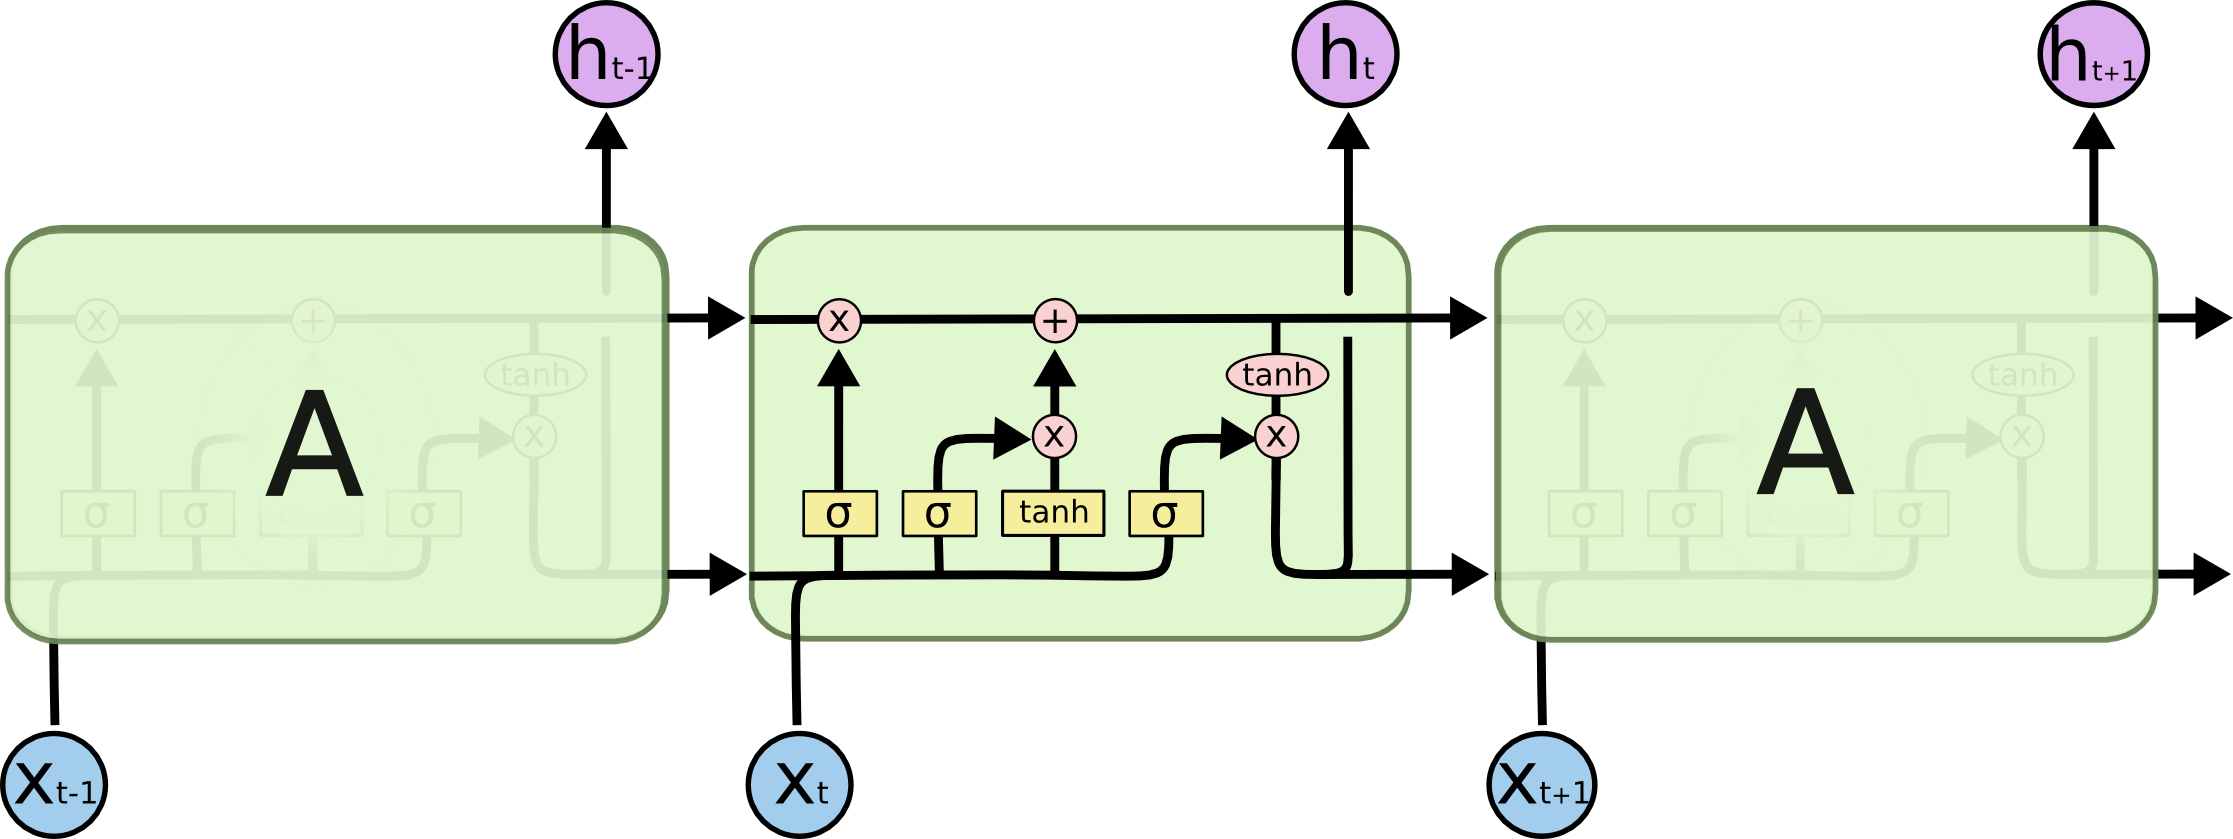
\includegraphics[width=\linewidth]{../../190813/figs/LSTM3-chain.png}

  \begin{itemize}
  \item Each cell gives an output and some additional information to the next cell
  \item Information from ordering of clustering algorithm extracted
  \item Allowed output to be a tensor with 12 features
  \item Dense network ran next to LSTM,
    and merged through one more dense layer
    to form final layer of output
  \end{itemize}

\end{frame}

\begin{frame}
  \frametitle{Training Specs}

  \begin{itemize}
  \item Trained with batch sizes of 10,000 jets
  \item The LSTM had the least training steps at 2,000, due to time constraints
    \begin{itemize}
    \item Continued to train while creating n-tuples
    \end{itemize}
  \item Other networks trained for 7,500 steps
  \item All can benefit from additional training time
  \end{itemize}

  \centering
  \includegraphics[width=0.5\linewidth]{190814_loss/plot_loss.pdf}

  Can be smoothed out by increasing batch size

\end{frame}

\begin{frame}
  \frametitle{Resolution of Signal Sample}

  \twofigs{$p_T$ targets}
          {190813_compare/comparison.pdf}
          {Direction targets}
          {190813_compare_direction/comparison.pdf}

  \begin{itemize}
  \item PUPPI information shifts peak the most
  \item Direction training does not look beneficial
  \end{itemize}

\end{frame}

\begin{frame}
  \frametitle{Resolution of Signal Sample}

  Fit a Bukin distribution over each training's di-jet mass peak

  \begin{center}
    \textcolor{blue}{Dense network with PUPPI, $p_T$ target}
    \includegraphics[width=0.5\linewidth]{190813_bukin/signal_hbb_m_190723_puppi.pdf}
  \end{center}

  Width for no training: $\sigma = 13.43 \pm 0.07$

  \vspace{12pt}

  \begin{columns}
    \begin{column}{0.5\linewidth}
      For $p_T$ targets:
      \begin{itemize}
      \item Original: $\sigma = 11.83 \pm 0.06$
      \item PUPPI: $\sigma = 11.80 \pm 0.06$
      \item PF Cands in LSTM: $\sigma = 12.22 \pm 0.06$
      \end{itemize}
    \end{column}
    \begin{column}{0.5\linewidth}
      For direction targets:
      \begin{itemize}
      \item Original: $\sigma = 13.43 \pm 0.07$
      \item PUPPI: $\sigma = 13.70 \pm 0.07$
        \phantom{\item PF Cands in LSTM: \\ $\sigma = 12.22$}
        \phantom{\item PF Cands in LSTM: \\ $\sigma = 12.22$}
      \end{itemize}
    \end{column}
  \end{columns}

\end{frame}

\begin{frame}
  \frametitle{Bukin Mean of Signal Sample}

  Mean for no training: $\mu = 120.8 \pm 0.1$

  \vspace{12pt}

  \begin{columns}
    \begin{column}{0.5\linewidth}
      For $p_T$ targets:
      \begin{itemize}
      \item Original: $\mu = 121.8 \pm 0.1$
      \item PUPPI: $\mu = 125.0 \pm 0.1$
      \item PF Cands in LSTM: $\mu = 124.5 \pm 0.1$
      \end{itemize}
    \end{column}
    \begin{column}{0.5\linewidth}
      For direction targets:
      \begin{itemize}
      \item Original: $\mu = 120.8 \pm 0.1$
      \item PUPPI: $\mu = 120.5 \pm 0.1$
        \phantom{\item PF Cands in LSTM: \\ $\mu = 12.22$}
        \phantom{\item PF Cands in LSTM: \\ $\mu = 12.22$}
      \end{itemize}
    \end{column}
  \end{columns}

  \vspace{24pt}

  PUPPI information gives best relative improvement

  \begin{itemize}
  \item No Training: $\frac\sigma\mu = 0.1111 \pm 0.0006$
  \item Original: $\frac\sigma\mu = 0.0971 \pm 0.0005$
  \item PUPPI: $\frac\sigma\mu = 0.0944 \pm 0.0005$
  \item LSTM: $\frac\sigma\mu = 0.0980 \pm 0.0005$
  \end{itemize}

\end{frame}


\begin{frame}
  \frametitle{Validation in Control Regions: Original Network}

  Original architecture agrees well

  \fourfigs{Z + b; high tag}
           {190813_validation/heavyz_jet1_tf_190723_origin_ptratio.pdf}
           {Z + b; low tag}
           {190813_validation/heavyz_jet2_tf_190723_origin_ptratio.pdf}
           {$t\bar{t}$; high tag}
           {190813_validation/tt_jet1_tf_190723_origin_ptratio.pdf}
           {$t\bar{t}$; low tag}
           {190813_validation/tt_jet2_tf_190723_origin_ptratio.pdf}

\end{frame}


\begin{frame}
  \frametitle{Validation in Control Regions: Original Network}

  PUPPI is behaving poorly in $t\bar{t}$

  \fourfigs{Z + b; high tag}
           {190813_validation/heavyz_jet1_tf_190723_puppi_ptratio.pdf}
           {Z + b; low tag}
           {190813_validation/heavyz_jet2_tf_190723_puppi_ptratio.pdf}
           {$t\bar{t}$; high tag}
           {190813_validation/tt_jet1_tf_190723_puppi_ptratio.pdf}
           {$t\bar{t}$; low tag}
           {190813_validation/tt_jet2_tf_190723_puppi_ptratio.pdf}

\end{frame}


\begin{frame}
  \frametitle{Differences in Analysis Sensitivity}

  Performed a rough sensitivity analysis using 2018 data

  \begin{itemize}
  \item Zero lepton selection and control regions
  \item Cutting on adjusted di-jet $p_T$
  \item Using lower deepCSV value of dijet for CRs
  \item Fitting mass for signal region
  \item Very little constraint on W + jets
  \item Few systematics: \\ luminosity, pileup, and diboson uncertainties
  \end{itemize}

  Expected significances

  \centering
  \begin{tabular}{l | r | r}
    Model & 50\% & 97.5\% \\
    \hline
    No training & 1.82 & 3.45 \\
    Original & 1.73 & 3.25 \\
    PUPPI & 1.71 & 3.22 \\
    LSTM & 1.73 & 3.29
  \end{tabular}

\end{frame}

\begin{frame}
  \frametitle{Conclusions}

  For 2018 data and MC:

  \begin{itemize}
  \item PUPPI information brings improvement on top of information used in 2016/2017 training
  \item Theoretically, LSTM should perform better,
    but initial results do not suggest there is much to gain
  \item Training for direction only does not help
  \end{itemize}

  Action list:

  \begin{itemize}
  \item Train all achitectures longer and with previous Huber loss $\delta$
  \item Determine how many PUPPI variables can be removed
  \item Apply direction change on top of $p_T$ regression
  \end{itemize}

\end{frame}

\beginbackup

\begin{frame}
  \frametitle{Backup Slides}
\end{frame}

\begin{frame}
   \frametitle{\small 190611/plot\_time\_60000\_wide}
   \centering
   \includegraphics[width=0.6\linewidth]{190611/plot_time_60000_wide.pdf}
\end{frame}

\begin{frame}
   \frametitle{\small 190611/plot\_time\_wide}
   \centering
   \includegraphics[width=0.6\linewidth]{190611/plot_time_wide.pdf}
\end{frame}

\begin{frame}
   \frametitle{\small 190611/plot\_time\_120000\_compare}
   \centering
   \includegraphics[width=0.6\linewidth]{190611/plot_time_120000_compare.pdf}
\end{frame}

\begin{frame}
   \frametitle{\small 190611/plot\_time\_60000\_compare}
   \centering
   \includegraphics[width=0.6\linewidth]{190611/plot_time_60000_compare.pdf}
\end{frame}

\begin{frame}
   \frametitle{\small 190611/plot\_time\_80000\_compare}
   \centering
   \includegraphics[width=0.6\linewidth]{190611/plot_time_80000_compare.pdf}
\end{frame}

\begin{frame}
   \frametitle{\small 190611/plot\_time\_120000\_narrow}
   \centering
   \includegraphics[width=0.6\linewidth]{190611/plot_time_120000_narrow.pdf}
\end{frame}

\begin{frame}
   \frametitle{\small 190611/plot\_time\_40000\_narrow}
   \centering
   \includegraphics[width=0.6\linewidth]{190611/plot_time_40000_narrow.pdf}
\end{frame}

\begin{frame}
   \frametitle{\small 190611/plot\_time\_160000\_narrow}
   \centering
   \includegraphics[width=0.6\linewidth]{190611/plot_time_160000_narrow.pdf}
\end{frame}

\begin{frame}
   \frametitle{\small 190611/plot\_time\_60000\_narrow}
   \centering
   \includegraphics[width=0.6\linewidth]{190611/plot_time_60000_narrow.pdf}
\end{frame}

\begin{frame}
   \frametitle{\small 190611/plot\_time\_80000\_narrow}
   \centering
   \includegraphics[width=0.6\linewidth]{190611/plot_time_80000_narrow.pdf}
\end{frame}

\begin{frame}
   \frametitle{\small 190611/plot\_time\_narrow}
   \centering
   \includegraphics[width=0.6\linewidth]{190611/plot_time_narrow.pdf}
\end{frame}



\backupend

\end{document}
